\documentclass[a4paper,10pt]{article}
\usepackage{float}
\usepackage{fancyhdr}
\usepackage{graphicx}
\usepackage{geometry}
\geometry{a4paper, left=2cm, right=2cm, top=1.5cm, bottom=3cm }
\usepackage{caption}
\usepackage{algorithm}
\usepackage{amsmath}
\DeclareMathOperator*{\argmax}{argmax}
\usepackage{subcaption}
\usepackage[hidelinks]{hyperref}
\usepackage{natbib}
\usepackage{xcolor}
\usepackage{etoolbox,fancyhdr,xcolor}
\newcommand{\headrulecolor}[1]{\patchcmd{\headrule}{\hrule}{\color{#1}\hrule}{}{}}
\newcommand{\footrulecolor}[1]{\patchcmd{\footrule}{\hrule}{\color{#1}\hrule}{}{}}
\renewcommand{\headrulewidth}{0.2pt}
\renewcommand{\footrulewidth}{0.2pt}
\usepackage{algpseudocode}

\fancyhead{} % clear all header fields
\fancyhead[L]{Automatic Image Captioning With Transformers}
\fancyfoot{} % clear all footer fields
\fancyfoot[R]{\thepage}
\fancyfoot[L]{Artificial Intelligence and Data Science}

\setlength{\headheight}{15mm}
\pagestyle{fancy}

\bibliographystyle{apalike}
\usepackage{times}
\usepackage{biblatex}
\addbibresource{references.bib}
\begin{document}
\begin{titlepage}
	\setlength{\parindent}{0pt}
	\large
\centering
\includegraphics[width=0.15\textwidth]{./esi-sba.png} \\
\vspace{0.5cm}
Ministry of Higher Education and Research \par
Higher School of Computer Science 08 May 1945 - Sidi Bel Abbes \par
\vspace{0.5cm}
Second Year Second Cycle - Artificial Intelligence and Data Science
\vspace{5cm}
\hrule
\vspace{0.5cm}
{\large Project Report\par}

\vspace{0.25cm}
{\LARGE\scshape Automatic Image Captioning with transformers\par}

\vspace{0.75cm}
\hrule

\vfill

\begin{minipage}[t]{.5\linewidth}
	Students: \vspace{0.25cm}\\
	• Abdelnour FELLAH \\
	• Abderrahmene BENOUNENE \\
	• Adel Abdelkader MOKADEM \\
        • Meriem MEKKI\\
	• Yacine Lazreg BENYAMINA \\
\end{minipage}%
\begin{minipage}[t]{.5\linewidth}
	\raggedleft
	Supervisor:\vspace{0.25cm}\\
	Dr. Rabab Bousmaha
\end{minipage}

\vspace{4cm}
\raggedright
Release date: \today
\end{titlepage}

\newpage
\renewcommand{\contentsname}{\begin{center}{Table of contents}\end{center}}
\tableofcontents
\newpage
\renewcommand{\contentsname}{\begin{center}{Table of figures}\end{center}}
\listoffigures
\newpage
\renewcommand{\contentsname}{\begin{center}{Table of tables}\end{center}}
\listoftables
\newpage

\section{\scshape{Introduction}}

\noindent Automatic image captioning is a multidisciplinary task that combines computer vision and natural language processing techniques to construct deep learning systems capable of generating textual descriptions for images. The significance of solving this task lies in its potential to cater to individuals with impaired vision. An effective AI Image Captioning System can be -for example- integrated into websites and mobile applications to enhance accessibility.\\

\noindent The problem of automatically generating a caption for a given image is considered an end-to-end sequence-to-sequence problem. This is because it takes an image, which is a sequence of pixels, and produces a caption, which is a sequence of tokens, without the need for manual feature extraction. The model processes the entire image to produce the entire output sequence, with minimal pre- or post-processing required.\\

\noindent In this report, we will elaborate on our approach using an Encoder-Decoder architecture based on transformers and vision transformers to construct a model capable of generating captions for images. The source code for the project can be accessed at: \textcolor{blue}{\href{https://github.com/Devnetly/image-captioning}{https://github.com/Devnetly/image-captioning}}.

\section{\scshape{Encoder-Decoder Architecture}}

\noindent An Encoder-Decoder is a type of neural network architecture used in sequence-to-sequence learning. It comprises two main components: an \textbf{encoder} and a \textbf{decoder}. This architecture enables various tasks, including machine translation, text-to-speech, speech-to-text, and image captioning.\\

\noindent \textbf{The encoder} part takes the input sequence,process it and produces a context vector/or a set of context vectors which are then fed to \textbf{The decoder} part that which takes the the encoder's output and tries to construct the output sequence, the encoder and decoder parts are task-dependent for example in the case of machine translation both the encoder and decoder parts are RNN-based networks.\\

\noindent Attention mechanisms are usually used with Encoder-Decoder architectures to enhance the model's ability to capture complex relationships between the input and output sequences.

\begin{figure}[H]
    \centering
    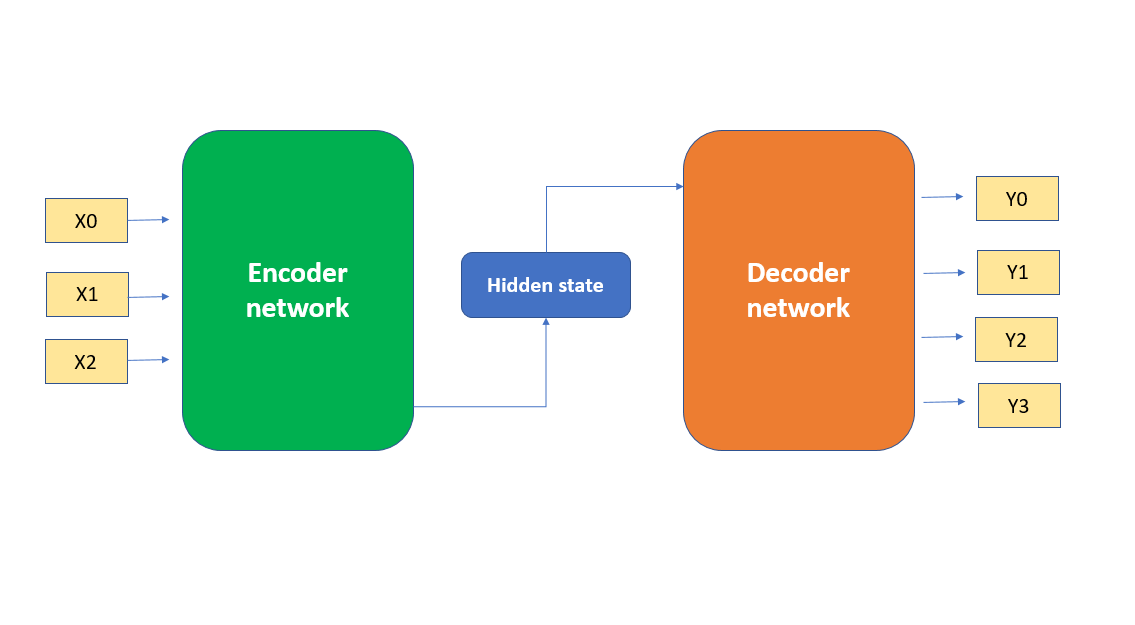
\includegraphics[width=0.8\textwidth]{NLP/figures/encoder-decoder-architecture.png}
    \caption{Encoder-Decoder Architecture, \textcolor{blue}{\href{https://vitalflux.com/encoder-decoder-architecture-neural-network/}{source}}.}
    \label{fig:enter-label}
\end{figure}

\newpage

\section{\scshape{Transformers}}

\noindent Transformers, introduced in 2017 by Google in their paper Attention is All You Need \cite{DBLP:journals/corr/VaswaniSPUJGKP17}
 are a \textbf{encoder-decoder} architecture designed for sequence-to-sequence tasks. They leverage multi-head attention mechanisms to handle long-range dependencies more effectively than previous models. Transformers have become foundational in natural language processing, excelling in tasks such as machine translation, text generation, and language understanding.

\begin{figure}[H]
    \centering
    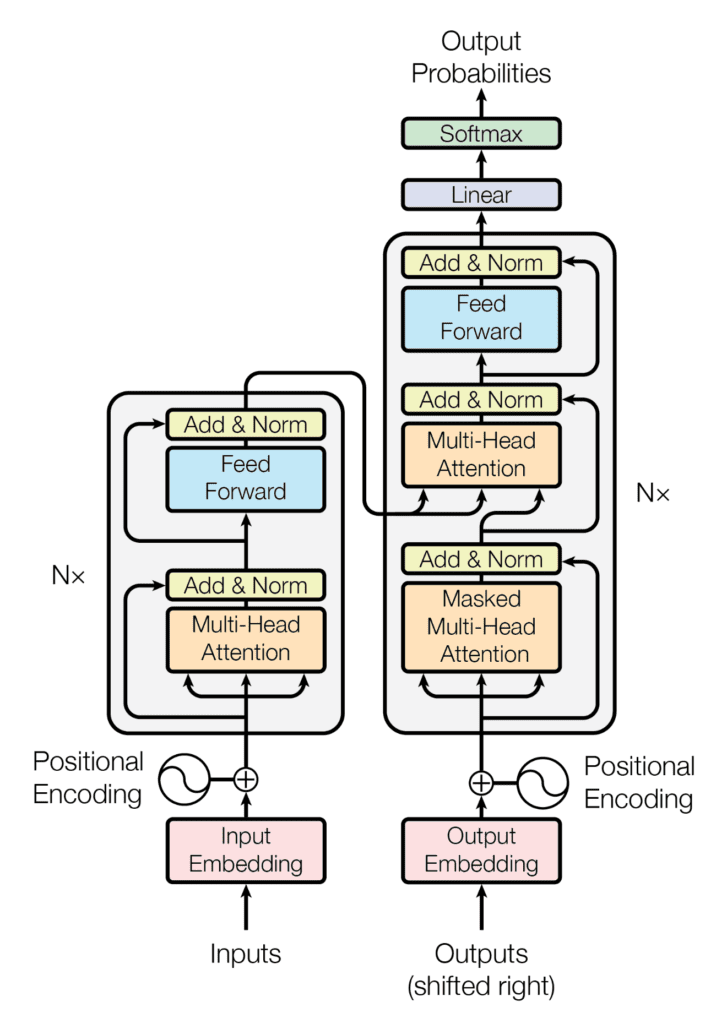
\includegraphics[width=0.4\textwidth]{NLP/figures/transformer.png}
    \caption{The transformer architecture, \textcolor{blue}{\href{https://arxiv.org/pdf/1706.03762}{source.}}}
    \label{fig:enter-label}
\end{figure}

\noindent A transformer consists of N encoder and decoder layers. The first encoder layer takes as input the token embeddings with positional encoding, while subsequent encoder layers operate on the output of the previous encoder.\\

\noindent The first decoder layer takes as input the token embeddings with positional encoding of the output sequence as well as the output of the last encoder layer, while subsequent decoder layers operate on the output of the previous decoder layer as well as the output of the last encoder layer.\\

\noindent The outputs of the last decoder layer are then passed through a linear layer to map them to the dimension of the output sequence (the size of the vocabulary of the output sequences). Finally, softmax is applied to generate probabilities.

\subsection{\scshape{Embedding Layer}}

\noindent An Embedding Layer is essentially used to represent categorical/discrete features as continuous vectors. In NLP, embedding layers are used to represent each token in the vocabulary with a vector. The weight of an embedding layer is a matrix of dimension 
$V \times D$, where $V$ is the size of the vocabulary and $D$ is the dimension of the vector. Therefore, an embedding layer takes a sequence of length $S$ and produces a matrix of dimensions $S \times D$.\\

\noindent The weight matrix is either initialized randomly and updated through backpropagation, or initialized with precomputed vectors such as GloVe, or a combination of both.

\newpage
\subsection{\scshape{Positional Encoding}}

\noindent Since transformers process the entire input sequence at the same time unlike recurrent units a form of ordering is needed in the architecture as it is clear that meaning of the sequences can change by changing the order of its elements.\\

\noindent A positional encoding layer maps each unique index to a vector of dimension $D$,so the weight of a positional encoding layer is a $S \times D$ matrix $W$ where $S$ is the size length of the input sequence and $D$ is the dimension of the embedding vectors,it takes an input $x$ of dimension $S \times D$,and produces the output $y = x + W$.\\

\noindent The weights of the positional encoding layer are not learnable and remain fixed; they are not updated during backpropagation, and they are initialized using the following formula :

$$
\begin{cases}
    W_{i,2 * j} = sin(\frac{i}{\frac{2 * j}{N^D}}) \\
    W_{i,2 * j + 1} = cos(\frac{i}{\frac{2 * j}{N^D}})
\end{cases}
$$

\noindent The value of $N$ is usually set to $10000$.

\subsection{\scshape{Multi-Head Attention \& Masked Multi-Head Attention}}

\begin{figure}[H]
    \centering
    \begin{subfigure}[b]{0.25\textwidth}
        \centering
        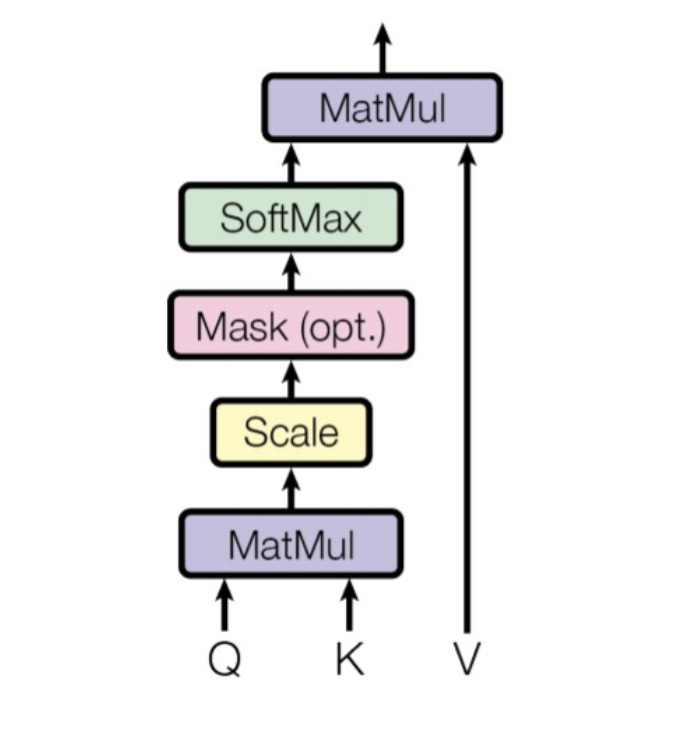
\includegraphics[width=\textwidth]{NLP/figures/scaled-dot-product.png}
        \caption{Scaled-Dot-Product}
    \end{subfigure}
    \begin{subfigure}[b]{0.25\textwidth}
        \centering
        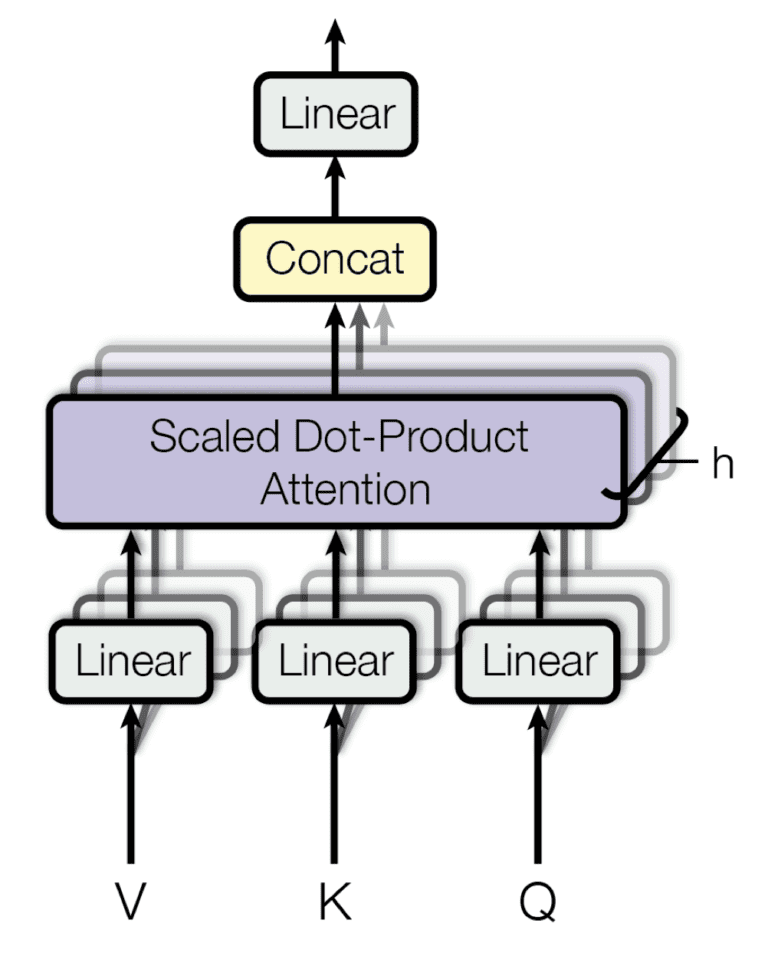
\includegraphics[width=\textwidth]{NLP/figures/multi-head-attention-2.png}
        \caption{Multi-Head-Attention}
    \end{subfigure}
    \caption{Multi-Head-Attention Mechanism}
\end{figure}

\subsubsection{\scshape{Self-Attention}}

\noindent\textbf{{\scshape{Value,Key and Query : \\}}}

\noindent A self-attention (or single-headed attention) layer is mainly composed of three linear layers called Value, Key, and Query, respectively. Their weights are all of dimension $D \times D_{\text{att}}$. Each layer is used to map the values of the input matrix (token embeddings + positional encoding) and/or change its dimension, meaning that each layer outputs a matrix of dimensions $S \times D_{\text{att}}$,lets call the resulted matrices $V_{output},K_{output}$ and $Q_{output}$ respectively .\\

\noindent\textbf{{\scshape{Scaled Dot-Product : \\}}}

\noindent Then in \textbf{MatMul} stage the matrices $V_{output},K_{output}$ are multiplied,$y = Q_{output} \times V_{output}$, resulting in a $S \times S$ matrix that is  often called \textbf{Attention Filter} which can be viewed as the attention that each token in the sequence is paying to other words in the sequence.\\


\noindent The attention scores are then scaled by dividing them by $\sqrt{S}$. This scaling is applied to prevent the issue of vanishing gradients. The scaled scores are then passed through a softmax layer to ensure that the values in each row of the attention matrix sum up to 1.\\

\noindent The attention Filter is then multiplied by the $V_{output}$ matrix to produce a matrix of dimension $S \times D_{att}$.

$$
ScaledDotProduct(Q,K,V) = softmax(\frac{Q\times K^T}{\sqrt{S}}) \times V
$$

\subsubsection{\scshape{Multi-Head Attention}}

\noindent Unlike self-attention,multi-head attention learns multiple filters instead of one using the same mechanism described previously,so it can be viewed to a $h$ self-attention layers with an output dimension $D_{att} / h$ where $h$ is the number of heads.\\

\noindent The outputs of the Scaled Dot-Product stage of each head are then concatenated resulting in an $S \times D\_att$ matrix,this matrix is then finally passed to fully connected layer which maps the values and changes input dimension back to $S \times D$.

\subsubsection{\scshape{Masked Multi-Head Attention}}

\noindent You may have noticed that in the figure above, a mask stage can be optionally performed after the Scale stage. The role of this stage is to prevent the model from looking into the future (i.e., paying attention to next tokens in the sequence) by masking (setting to zero) the upper triangular part of the attention filter.

\subsection{\scshape{Add \& Norm Layer}}

\subsubsection{Add}

\noindent The add layer (also known ad skip-connection or residual-connection) preforms element-wise addition between the input and the output of the previous layer,which helps preventing the issue of vanishing gradient descent and allows for a better information flow.

\subsubsection{Norm}

\noindent After the addition operation, layer normalization is applied. Layer normalization normalizes the values across the feature dimension for each example in the mini-batch. This helps in stabilizing the learning process and improving generalization.

\section{\scshape{Vision Transformers}}

\noindent Vision transformers are encoder-only transformers adapted for computer vision tasks. The idea is to break down an image of size $W \times H$ into a series of patches of size $P_w \times P_h$. These patches are then flattened, resulting in a two-dimensional matrix of dimensions $S \times D$, where $S = \frac{W}{P_w} \times \frac{H}{P_h}$ and $D = P_w \times P_h$. A linear projection layer is used to transform the individual flattened patches to a lower-dimensional vector, resulting in a matrix of dimension $S \times D'$. Finally, positional embedding is applied.\\

\noindent The output of patching and positional embedding is then fed to a regular transformer encoder,the outputs of the encoder are then passed to a Multi-Layer Perception to output the classes probabilities. 

\begin{figure}[H]
    \centering
    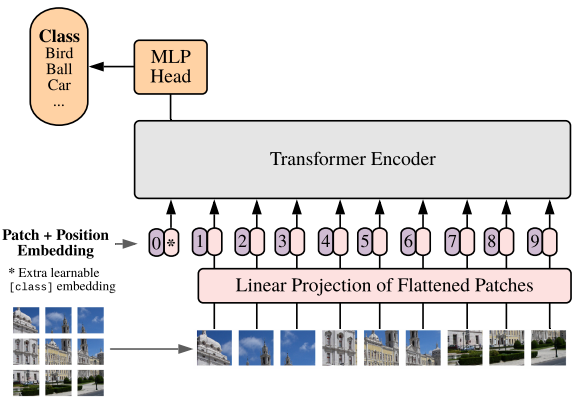
\includegraphics[width=0.6\textwidth]{NLP/figures/vision-transformer.png}
    \caption{Vision Transformer, \textcolor{blue}{\href{https://paperswithcode.com/method/vision-transformer}{source.}}}
    \label{fig:enter-label}
\end{figure}

\newpage

\section{\scshape{DieT : Data Efficient Image Transformer}}

\noindent DIET, introduced in 2021 by Facebook AI, stands for Data Efficient Image Transformer. It enhances the classic Vision Transformer to reduce the requirement for vast amounts of training data and the computational requirements of the model using A \textbf{teacher-student} with \textbf{distillation} token, the student model is first trained to mimic the teacher's behaviour then further fine-tuned on the original task using the ground truth labels.\\

\noindent\subsection{\scshape{Soft Distillation}}

$$
\mathcal{L} = (1 - \lambda) * \mathcal{L}_{ce}(f(Z_{s}),y) + \lambda * \tau ^ 2 * KL(f(\frac{Z_{t}}{\tau}), f(\frac{Z_{s}}{\tau})))
$$

\noindent where : 

\begin{itemize}
    \item $Z_{s}$ : the student's logits.
    \item $Z_{t}$ : the teacher's logits.
    \item $\lambda$ : coefficient balancing KL divergence and cross entropy loss,between 0 and 1.
    \item $\tau$ : The temperature (Distillation).
    \item $\mathcal{L}_{ce}$ : The cross entropy loss function.
    \item $f$ : the student.
\end{itemize}

\noindent\subsection{\scshape{Hard Distillation}}

$$
\mathcal{L} = \frac{1}{2} \mathcal{L}_{ce}(f(Z_{s}), y) + \frac{1}{2} \mathcal{L}_{ce}(f(Z_{s}), y_{t})
$$

\noindent where : 

\begin{itemize}
    \item $y_{t}$ : the tachers's predictions.
    \item $y$ : the real labels.
\end{itemize}

\noindent\subsection{\scshape{Distillation Token}}

\noindent A special token called distillation token is added,and it is learnable through back propagation,it represents and capture the knowledge transferred from the larger teacher model during the knowledge distillation process.

\begin{figure}[H]
    \centering
    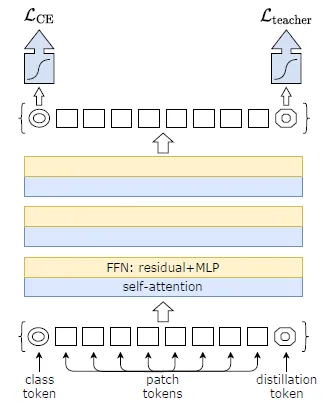
\includegraphics[width=0.3\textwidth]{NLP/figures/distillation_token.png}
    \caption{Distillation Process, \textcolor{blue}{\href{https://miro.medium.com/v2/resize:fit:640/format:webp/1*F-gCWtXEMsUlA10HSeQoSw.png}{source.}}}
\end{figure}

\newpage
\section{\scshape{Architecture}}

\noindent For this task, we chose an Encoder-Decoder architecture with a \textbf{DeiT-III} (with the last classification layer) in the encoder part and a Transformer decoder in the decoder part, with an additional fully connected layer to output class probabilities.

\begin{figure}[H]
    \centering
    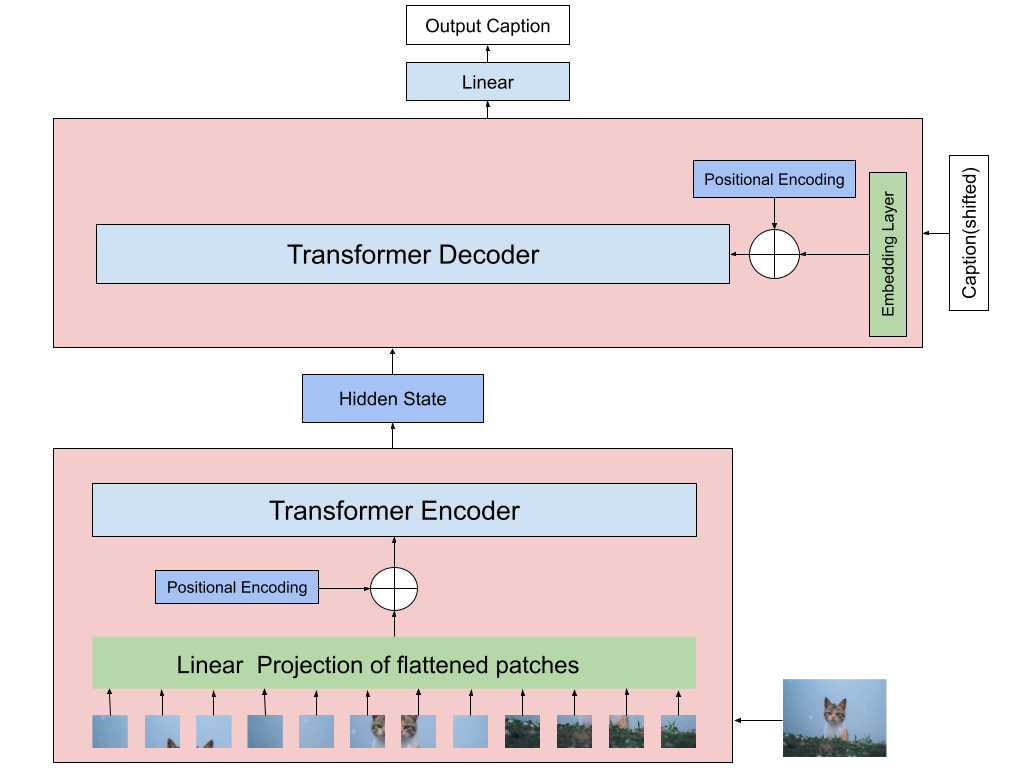
\includegraphics[width=\textwidth]{NLP/figures/architecture.png}
    \caption{The model's architecture.}
\end{figure}

\section{\scshape{Dataset}}

\noindent The dataset used to train the model is the \textcolor{blue}{\href{https://www.kaggle.com/datasets/eeshawn/flickr30k}{Flickr30k}} dataset with \textbf{31,783} images of various resolutions and five captions per image, totaling \textbf{158,915} image-caption pairs. The dataset size is \textbf{4.39GB} and primarily consists of images depicting people involved in everyday activities and events,the dataset does not provide any predefined split, so we divided it into a training and a test set with ratios of 0.8 and 0.2, respectively. while ensuring that all captions for the same image are in the same set.\\

\begin{figure}[H]
    \centering
    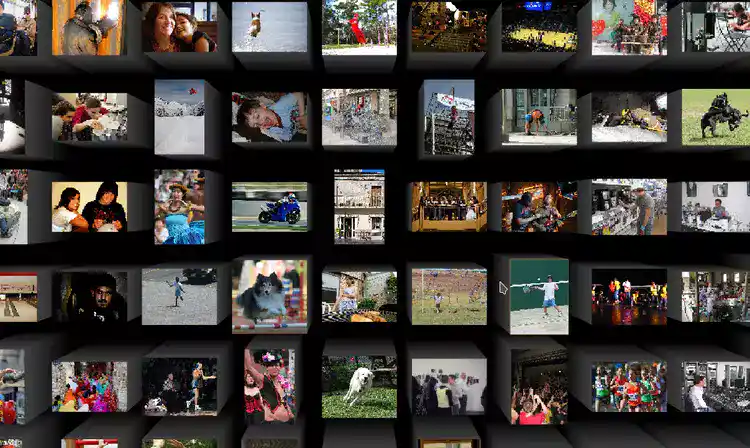
\includegraphics[width=0.8\textwidth]{NLP/figures/flickr30k-dataset.png}
    \caption{The Flickr30k Dataset, \textcolor{blue}{\href{https://datasets.activeloop.ai/docs/ml/datasets/flickr30k-dataset/}{source.}}}
    \label{fig:enter-label}
\end{figure}

\newpage

\section{\scshape{Preprocessing \& Data Augmentation}}

\subsection{\scshape{Images Preprocessing \& Augmentation}}

\noindent At training, the input images were randomly horizontally flipped, and then a random sub-image of size $384 \times 348$ pixels was randomly selected. The pixel values were divided by 255 as a form of normalization. At inference time, the images were all resized to a uniform resolution of $384 \times 384$ pixels, and the pixel values were divided by 255.

\subsection{\scshape{Captions Preprocessing}}

\noindent Before feeding the captions to the transformer, three steps of text normalization are applied: lowercasing, punctuation removal, and replacing multiple spaces with one space. The normalized captions are then tokenized using space-and-punctuation-based tokenization. Each token is replaced by its index in the vocabulary. To reduce the size of the vocabulary, a token has to appear in at least $n$ documents to be added to the vocabulary (in this case, we chose $n$ to be equal to 8). If a token is not found in the vocabulary, it will be replaced by the index of a special token called the unknown token. Additionally, special tokens representing the start and end of each sentence are appended to the beginning and end of each caption. Finally, the sequences are padded to all have the same length of 80.\\

\noindent The input sequences fed to the model are right-shifted (the last token in the sequence is removed). Meanwhile, the model is expected to predict the left-shifted caption (without the first token). This approach encourages the model to predict the next word based on the preceding words and the input image.

\section{\scshape{Metrics \& Evaluation}}

\subsection{Automatic evaluation}

\subsubsection{Perplexity}

\noindent  the perplexity metric in NLP quantifies the level of uncertainty a model exhibits when predicting or assigning probabilities to text, the lower the perplexity, the better the model is, The perplexity of the model q on a test sample $x_{1},x_{2},....,x_{N}$ is given.

$$
PPL(X) = (\prod\limits_{i=1}^{N} q(x_{i}))^{-\frac{1}{N}}
$$

\subsubsection{BLUE score (Bilingual Evaluation Understudy)}

\noindent BLUE (bilingual evaluation understudy) is a metric used to evaluate the generated text of machine translation models or models that are trying to solve similary task ,it was invented in 2001 at \textcolor{blue}{\href{https://en.wikipedia.org/wiki/IBM}{IBM}},it is known for having a high correlation with human annotations.\\

\noindent The BLUE score compares separate parts of a text with a set of
reference texts, and assigns a score to each part then these scores are averaged to give the final score, the higher the score, the better the model.

$$
BLUE Score = Brevity Penalty * Geometric Average Precision Score
$$

\noindent\textbf{\scshape{\\ Brevity Penalty : \\}}

\noindent The Brevity Penalty is included to prevent the score from giving a false impression of the model's performance by favoring very short sequences.

$$
Brevity Penalty = \begin{cases}
    1 \text{ if $c > r$}\\
    e^{1 - \frac{r}{c}} \text{ otherwise.}
\end{cases}
$$

\noindent Where $c$ is the length of the predicted text and $r$ is the length of the target text.

\newpage
\noindent\textbf{\scshape{\\ n-gram precision score : \\}}

$$
precision_{i} = \frac{\sum\limits_{snt \in Condidates} \sum\limits_{i \in snt} min(m_{cand}^{i}, m_{ref}^{i})}{w_{t}^{i} = \sum\limits_{snt \in Condidates} \sum\limits_{i' \in snt} m_{cand}^{i'}}
$$

\noindent where : 

\begin{itemize}
    \item $m_{cand}^{i}$  : This number of i-grams in the translation corresponds to the translation of the reference.
    \item $m_{ref}^{i}$ : the number of i-grams in the reference translation.
    \item $w_{t}^{i}$ : The total number of i-grams in the automatic translation.
\end{itemize}

\noindent\textbf{\scshape{\\ Geometric Average Precision Score : \\}}

$$
Geometric Average Precision Score = \prod\limits_{i=1}^{N} p_{i} ^ {w_{i}}
$$

\noindent Where $p_{i}$ is the precision score of the predicted text with $N = i$ ,and $w_{i}$ is its weight usually equal to $1 / N$.

\subsubsection{ROUGE score (Recall-Oriented Understudy for Gisting Evaluation)}

\noindent ROUGE, or Recall-Oriented Understudy for Gisting Evaluation, is a metric used to measure the similarity between a machine-generated summary and reference summaries. It does so by comparing overlapping n-grams. ROUGE scores range from 0 to 1, with higher scores indicating a greater similarity between the automatically generated summary and the reference summaries.

\noindent Mainly three variants of the ROUGE Score exists : \textbf{ROUGE-1} which uses unigrams,\textbf{ROUGE-2} which uses bigrams and \textbf{ROUGE-L} which uses longest common subsequence (LCS) : for each score a precision,recall and an f1-score can be calculated using the following formulas : 

$$
\begin{cases}
    ROUGE-N_{recall} = \frac{\mid N-grams_{cand} \cap N-grams_{ref} \mid}{\mid 
 N*grams_{ref} \mid}\\
 \noalign{\vskip9pt}
 ROUGE-N_{precision} = \frac{\mid N-grams_{cand} \cap N-grams_{ref} \mid}{\mid 
 N-grams_{cand} \mid}\\
 \noalign{\vskip9pt}
 ROUGE-N_{F1} = 2 * \frac{ROUGE-N_{recall} * ROUGE-N_{precision}}{ROUGE-N_{recall} + ROUGE-N_{precision}}
\end{cases}
$$

$$
\begin{cases}
    ROUGE-L_{recall} = \frac{LCS(cand, ref)}{\mid unigrams_{ref} \mid}\\
 \noalign{\vskip9pt}
 ROUGE-L_{recall} = \frac{LCS(cand, ref)}{\mid unigrams_{cand} \mid}\\
 \noalign{\vskip9pt}
 ROUGE-L_{F1} = 2 * \frac{ROUGE-N_{recall} * ROUGE-N_{precision}}{ROUGE-N_{recall} + ROUGE-N_{precision}}
\end{cases}
$$

\subsection{Human Evaluation}

\noindent In evaluation of translations, judges use a predefined scale, such as a 1 to 5 scale, where 1 represents the lowest and 5 the highest quality. However, defining clear descriptions for each score and distinguishing the levels of quality precisely can be challenging. Even with explicit guidelines, judges struggle to assign numerical values to translation quality. The evaluation focuses on two key metrics: adequacy and fluency.

\newpage
\section{\scshape{Training \& Results}}

\noindent The model's encoder was initialized using weights of pre-trained \textbf{DeiT-III} on the \textbf{ImageNet-22k} dataset,and we further fine-tuned it on our task instead of freezing it, while the decoder's weights were initialized randomly.\\

\noindent The model was trained for 11 epochs across three different sessions using the \textbf{AdamW} optimizer with learning rate of $10^{-4}$ and a weight decay of $10^{-4}$, a batch size of $8$ and a linear learning rate decay.\\

\noindent The training was done a NVIDIA GeForce RTX 3050 Ti Laptop GPU,and it took an average of 115 minutes per-epoch making the total training time 21 hours.

\begin{table}[!htb]
    % \caption{Global caption}
    \begin{minipage}{.5\linewidth}
        \centering
        \begin{tabular}{|l|l|}
            \hline
            \textbf{Hyper-parameter} & \textbf{Value} \\
            \hline
            Optimizer & AdamW \\
            Learning rate & $10^{-4}$\\
            Weight Decay & $10^{-4}$ \\
            Learning rate deacy & Linear Learning rate decay\\
            Batch size & 8\\
            \hline
        \end{tabular}
        \caption{Hyper-parameters}
    \end{minipage}%
    \begin{minipage}{.5\linewidth}
        \centering
        \begin{tabular}{|l|l|}
            \hline
            \textbf{Parameter} & \textbf{Value} \\
            \hline
            Features Diemenions & 256\\
            Patch size & 16 \\
            Heads count & 8\\
            Decoder Layer's count & 6\\
            Maximum Caption length & 80 \\
            \hline
        \end{tabular}
        \caption{The architecture's parameters.}
    \end{minipage} 
\end{table}

\subsection{\scshape{Learning graphs}}

\begin{figure}[H]
    \centering
    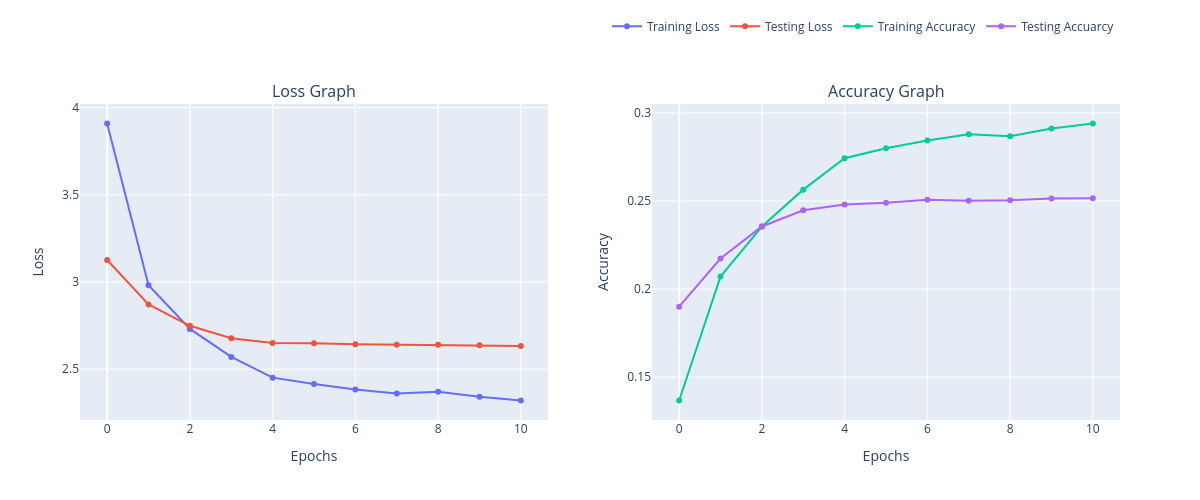
\includegraphics[width=0.9\textwidth]{NLP/figures/loss-accuracy.png}
    \caption{Loss & Accuracy}
    \label{fig:enter-label}
\end{figure}

\begin{figure}[H]
    \centering
    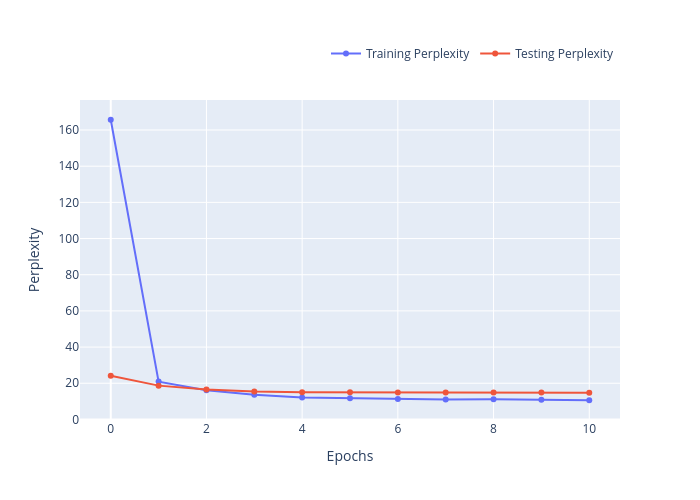
\includegraphics[width=0.5\textwidth]{NLP/figures/perplexity.png}
    \caption{Perplexity}
\end{figure}

\subsection{\scshape{Automatic Evaluation Results}}

\begin{table}[!htb]
    \begin{minipage}{.5\linewidth}
        \centering
        \begin{tabular}{|c|c|c|c|}
            \hline
            BLUE-1 & BLUE-2 & BLUE-3 & BLUE-4\\
            \hline
            0.6335 & 0.4656 & 0.3403 & 0.2451\\
            \hline
        \end{tabular}
        \caption{BLUE Score}
    \end{minipage}%
    \begin{minipage}{.5\linewidth}
        \centering
        \begin{tabular}{|c|c|c|c|}
            \hline
            & ROUGE-1 & ROUGE-2 & ROUGE-L\\
            \hline
            F1 & 0.5135 & 0.2569&	0.4728\\
            \hline
            Precision & 0.5477 &	0.274	& 0.5029\\
            \hline
            Recall & 0.5106 &	0.2576 &	0.4711\\
            \hline
        \end{tabular}
        \caption{ROUGE-Score}
    \end{minipage} 
    \caption{Automatic Evaluation Results}
\end{table}

\begin{figure}[!htb]
    \centering
    \begin{minipage}{.5\linewidth}
        \centering
        \begin{subfigure}[b]{\linewidth}
            \centering
            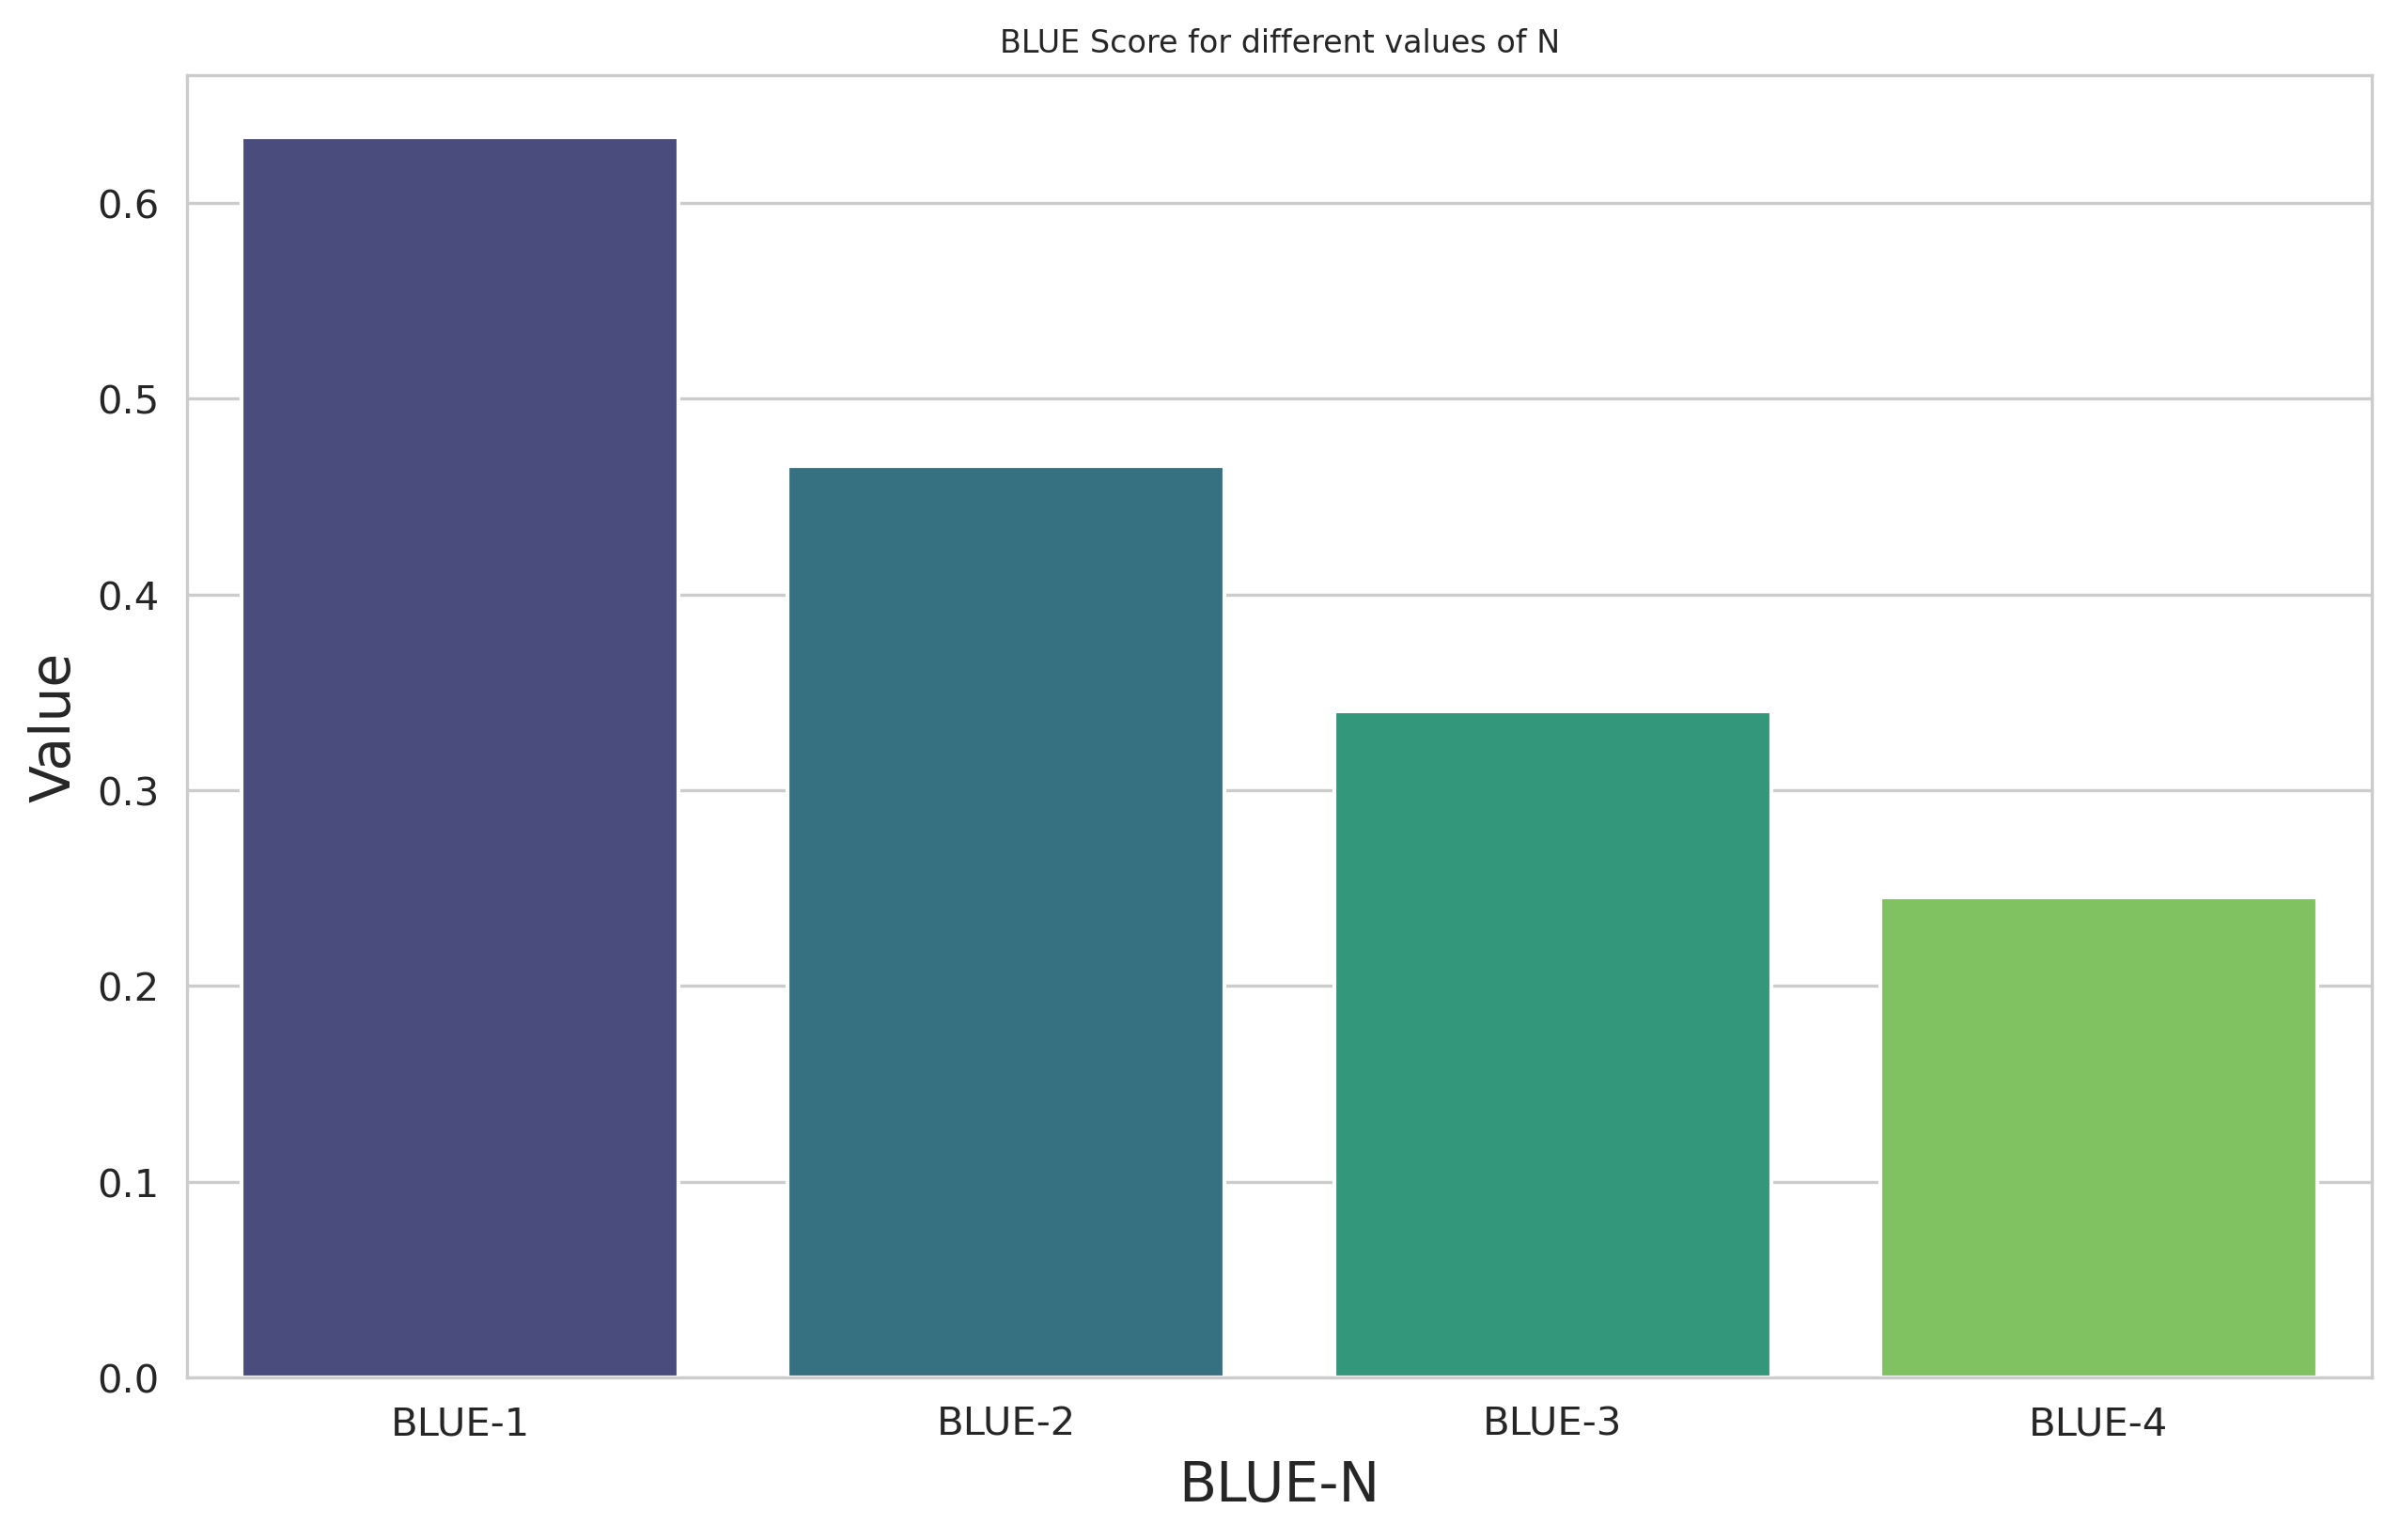
\includegraphics[width=\textwidth]{NLP/figures/blue_bar_plot.png}
            \caption{BLUE Score}
        \end{subfigure}
    \end{minipage}%
    \begin{minipage}{.5\linewidth}
        \centering
        \begin{subfigure}[b]{\linewidth}
            \centering
            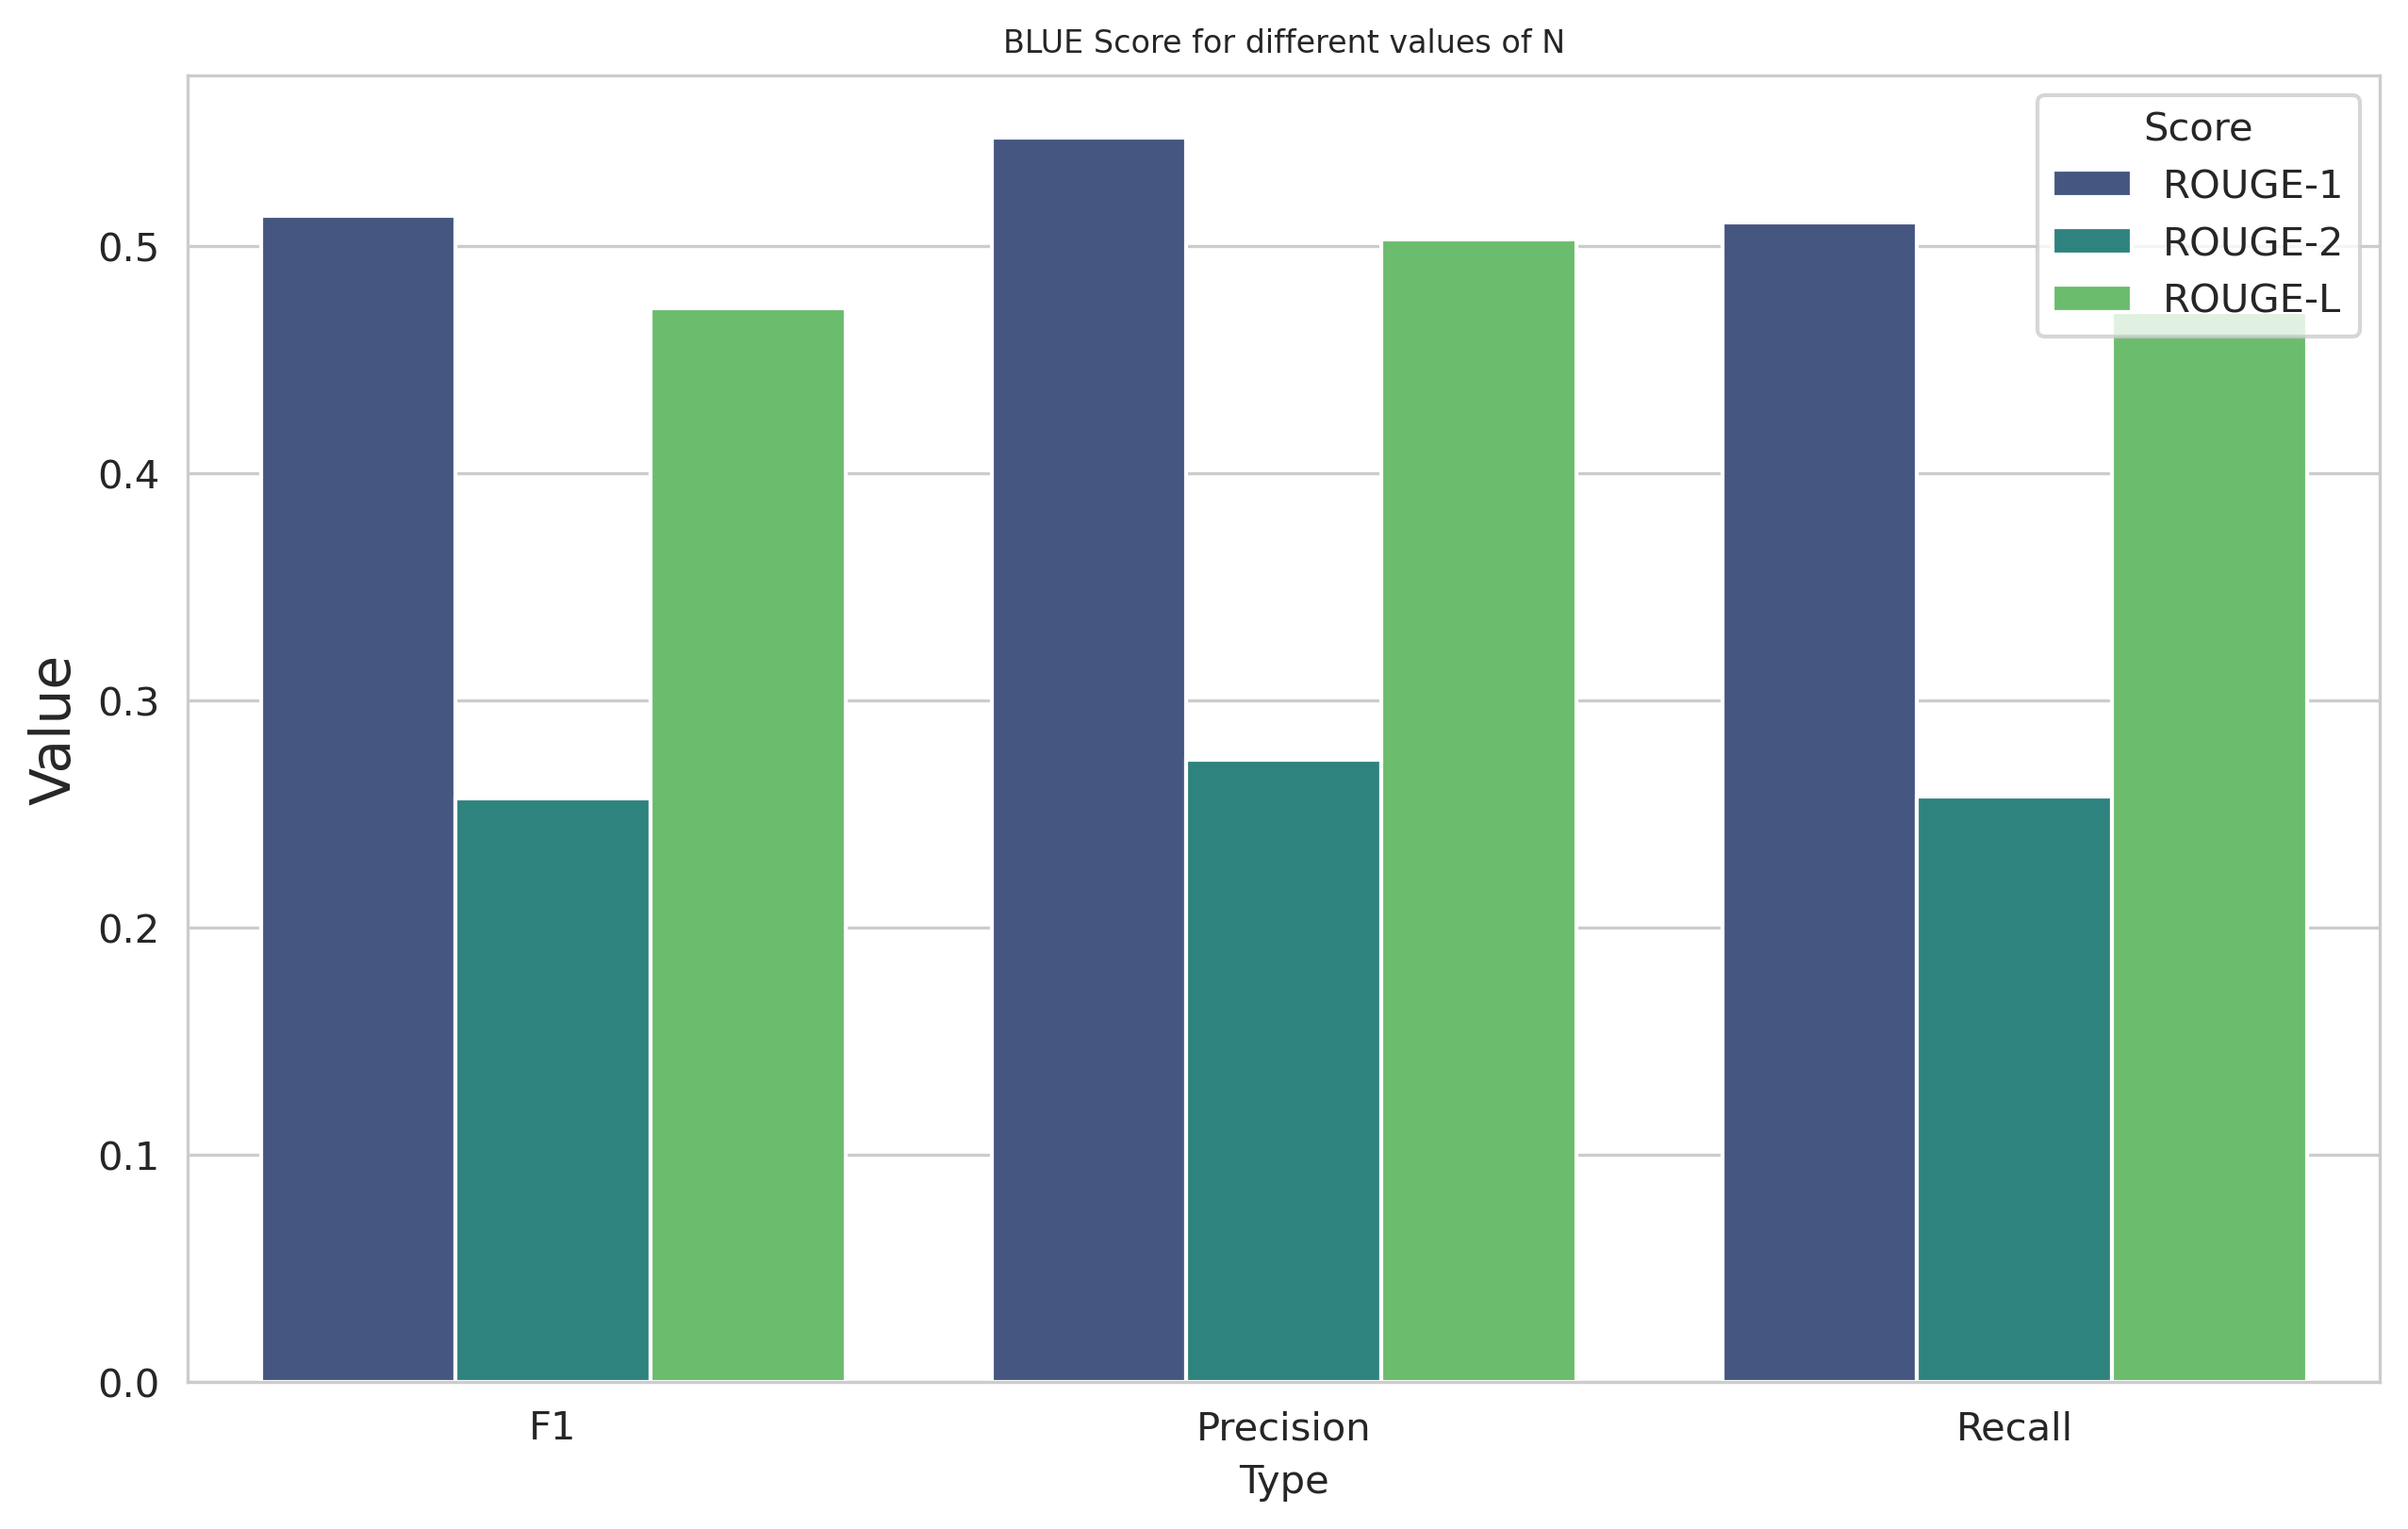
\includegraphics[width=\textwidth]{NLP/figures/rouge_bar_plot.png}
            \caption{ROUGE Score}
        \end{subfigure}
    \end{minipage}
    \caption{Automatic Evaluation Results}
\end{figure}


\subsection{\scshape{Testing on images outside of the dataset}}

\noindent To further test our model's ability to generalize on unseen data, we handpicked 20 images from the internet. These images contained similar objects to those in the training set but had different resolution ranges. Below are the results for some of them : 

\begin{figure}[H]
    \begin{center}
        \begin{tabular}{cc}
            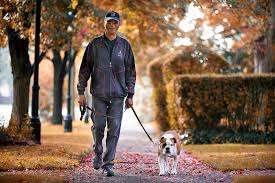
\includegraphics[width=68mm]{NLP/figures/test_results/01.jpeg} &   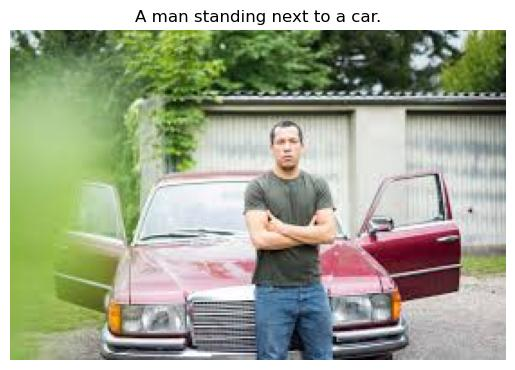
\includegraphics[width=50mm]{NLP/figures/test_results/16.jpeg} \\
            
             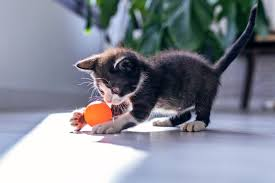
\includegraphics[width=58mm]{NLP/figures/test_results/14.jpeg} &   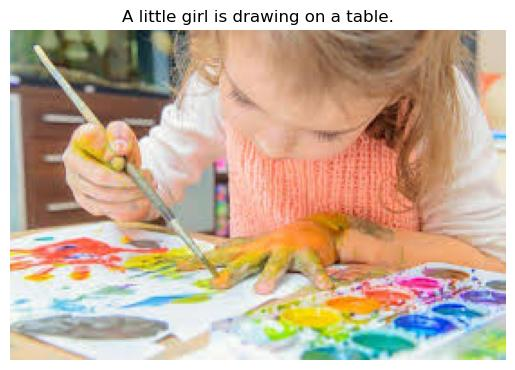
\includegraphics[width=54mm]{NLP/figures/test_results/08.jpeg}    
        \end{tabular}
    \end{center}
    \caption{The Generated captions}
\end{figure}

\newpage

\section{\scshape{Conclusion}}

\noindent In this project, we aimed to develop a model capable of generating captions for images using a transformer-based architecture. Our approach incorporated a Data-efficient Image Transformer (DeiT) as the encoder and a standard transformer decoder. We utilized the Flickr30k dataset for training and performed extensive text preprocessing alongside image resizing and augmentation to enhance the model's robustness.\\

\noindent Post-training evaluation was conducted using BLEU and ROUGE scores, and we also qualitatively assessed the model by generating captions for a variety of images randomly sourced from the internet. The results indicated that our model performed well on images similar to those in the training dataset, demonstrating its effectiveness in generating relevant captions. However, its performance declined on images that were significantly different from the training set, highlighting an area for improvement.\\

\noindent To further enhance the model's performance, several strategies can be considered. Expanding the dataset to include a more diverse set of images would likely improve the model's generalization capabilities. Experimenting with different model configurations and hyperparameters could also yield better results. Additionally, exploring advanced architectures, such as incorporating attention mechanisms or utilizing pre-trained models, may offer further improvements in caption generation quality.\\

\noindent Overall, while the current model shows promise, these suggested enhancements could significantly bolster its ability to generate accurate and contextually appropriate captions across a wider range of images.\\

\newpage

\section{\scshape{References}}

\nocite{DBLP:journals/corr/abs-2201-12944}
\nocite{DBLP:journals/corr/abs-2012-12877}
\nocite{young-etal-2014-image}
\printbibliography[heading=none]

\end{document}